%! Author = Runge
%! Date = 29-12-2023

% Preamble
\documentclass[a4paper,conference, draft, onecolumn]{IEEEtran}

% Packages
%! Author = Runge
%! Date = 29-12-2023

% Packages
\RequirePackage{clrscode4e}
\usepackage{amsmath}
% \usepackage{amsthm} \\ the proof environment clashes with the one in pf2.
\usepackage{amssymb}
\usepackage{amsbsy}
\usepackage{mathrsfs}
\usepackage{dsfont}
\usepackage{bbold}
\usepackage{booktabs}
\usepackage{tikz}
\usepackage{pf2}
\usepackage{thmtools, thm-restate}
\usepackage{stmaryrd}

% Packages with options set
\usepackage[hidelinks]{hyperref}
\usepackage[textsize=small,obeyDraft]{todonotes}
\usepackage[newfloat]{minted}
\usepackage[backend=biber,
    bibencoding=utf8,
    maxbibnames=20,
    style=ieee,
    citestyle=numeric-comp,
    url=false
]{biblatex}
\usepackage[acronym]{glossaries}

% Package setup
\setlength{\marginparwidth}{2cm} % todonotes width
\setminted{linenos, autogobble, breaklines, fontsize=\footnotesize, style=friendly, xleftmargin=1em, numbersep=5pt}
\addbibresource{bib/main.bib}

% Other setup and options
\declaretheorem{theorem}
\declaretheorem{lemma}
\declaretheorem{definition}
\newfloat{algorithm}{htb!}{lop}
\floatname{algorithm}{Algorithm}
\newcommand{\algorithmautorefname}{Algorithm}

\makeatletter
\providecommand{\bigsqcap}{%
  \mathop{%
    \mathpalette\@updown\bigsqcup
  }%
}
\newcommand*{\@updown}[2]{%
  \rotatebox[origin=c]{180}{$\m@th#1#2$}%
}
\makeatother

\makeglossaries

\tikzstyle{state} = [rectangle, minimum width=1.5cm, minimum height=1cm, text centered, draw=black, fill=white!30]
\tikzstyle{circle} = [ellipse, minimum width=1.5cm, minimum height=0.5cm, text centered, draw=black, fill=white!30]

%! Author = Runge
%! Date = 29-12-2023

\newacronym{aau}{AAU}{Aalborg University}
\newacronym{lp}{LP}{linear programming}

%! Author = Runge
%! Date = 29-12-2023

\title{Supporting Schema Creation}

\author{\IEEEauthorblockN{Anders Malta Jakobsen}
\IEEEauthorblockA{\textit{dept. of Computer Science} \\
\textit{AAU}\\
Aalborg, Denmark \\
amja23@student.aau.dk}\\
\IEEEauthorblockN{Lars Emanuel Hansen}
\IEEEauthorblockA{\textit{dept. of Computer Science} \\
\textit{AAU}\\
Aalborg, Denmark \\
leha20@student.aau.dk}
\and
\IEEEauthorblockN{Casper Ståhl}
\IEEEauthorblockA{\textit{dept. of Computer Science} \\
\textit{AAU}\\
Aalborg, Denmark \\
cstahl20@student.aau.dk}\\
\IEEEauthorblockN{Oliver Holmgaard}
\IEEEauthorblockA{\textit{dept. of Computer Science} \\
\textit{AAU}\\
Aalborg, Denmark \\
oholmg20@student.aau.dk}
\and
\IEEEauthorblockN{Daniel Runge Petersen}
\IEEEauthorblockA{\textit{dept. of Computer Science} \\
\textit{AAU}\\
Aalborg, Denmark \\
dpet20@student.aau.dk}\\
\IEEEauthorblockN{Sebastian Aaholm}
\IEEEauthorblockA{\textit{dept. of Computer Science} \\
\textit{AAU}\\
Aalborg, Denmark \\
saahol20@student.aau.dk}
}

% Document
\begin{document}
    \maketitle
    %! Author = Runge
%! Date = 29-12-2023

\IEEEtitleabstractindextext{%
    \begin{abstract}
        This paper presents an alternative to the framework presented in abstract interpretation applied to SQL, aiming to overcome a possible non-termination problem in Halder and Cortesi's work.
        Our alternative is a complete static dataflow analysis developed in the abstract interpretation framework.
        Our method resolves this non-termination issue by extending the abstraction of tables to the multiplicity of tuples.
        Additionally, we introduce new abstractions of the values using regular expressions for strings and union intervals for integers, as initially proposed by Cousot.
        Our analysis is informally proven to be sound and terminate reliably, providing a solid foundation for future research.
    \end{abstract}
    \begin{IEEEkeywords}
        Abstract Interpretation, Databases, Formal Verification, Program Analysis
    \end{IEEEkeywords}
}

    \section{Introduction}\label{sec:introduction}
Software analysis is a broad field encompassing a wide range of techniques and methodologies, each tailored to address specific aspects of software systems.
One such technique is value analysis, which focuses on the behavior of a program with respect to its input and output values~\cite{jackson_software_2000}.
Value analysis can be approached from various angles, including the consideration of meta-information like information flow or taint analysis.
While these approaches offer valuable insights into the behavior of a program, they often require detailed knowledge of the program's internal workings and are not always applicable to all types of software systems.
In this paper we use static program analysis, specifically abstract interpretation.

Abstract interpretation, first proposed by Cousot and Cousot in 1977~\cite{cousot_abstract_1977}, has emerged as a fundamental method for static program analysis.
Over the years, it has evolved into a versatile tool, finding applications across various programming paradigms and system architectures.
Its utility extends beyond traditional imperative programming to encompass object-oriented designs and concurrent systems~\cite{gustafsson_analyzing_2013, mine_static_2023}.
Abstract interpretation has played a pivotal role in analyzing a spectrum of program properties, from basic safety and liveness concerns to intricate security considerations~\cite{mastroeni_abstract_2011}.

Building upon this, Halder and Cortesi have expanded the application of abstract interpretation to domains like query languages~\cite{halder_abstract_2012}.
This paper continues in these footsteps, aiming to further explore and extend the capabilities of abstract interpretation within the context of query languages.


\subsection{Non-terminating Analysis}\label{subsec:non-terminating-analysis}
One problem with Halder and Cortesi is that the analysis they propose may not terminate.
To illustrate, consider the database schema \autoref{lst:motivate-sql} with the program in \autoref{lst:motivate-program}


\begin{listing}
    \begin{minted}{sql}
        CREATE TABLE account (
            name    TEXT,
            balance INT
        );
    \end{minted}
    \caption{A simple schema representing an account.}
    \label{lst:motivate-sql}
\end{listing}


\begin{listing}
    \begin{minted}{bash}
        while true do
            insert((name, balance), ("name", 1))
    \end{minted}
    \caption{A tiny program with nonterminating analysis.}
    \label{lst:motivate-program}
\end{listing}


Because the database context would continually change under Cortesi and Halder, the analysis would not terminate.
However, this doesn't have to be the case.
Extending the analysis to consider abstract tuples, not just abstract values, it is possible to have the analysis terminate for the program in \autoref{lst:motivate-program}.

\textbf{TODO:Show the contributions through a second example that runs through how we used the updated semantics. Move from method}


\subsection{Contributions}\label{subsec:contributions}
\todo[inline]{Casper says: These section (\ref{subsec:contributions}, \ref{subsec:related-work}, \ref{subsec:article-overview}) read like notes, I assume they are.}

Use Halder concretely for abstract interpretation

This paper builds on work of abstract interpretation of database queries by Cortesi and Halder.
Concretely, we use their work for analysing a database schema in relation to a program using the syntax they describe.


Improve on the levels of abstraction, i.e., add not just abstract values but also abstract tuples

Describe an implementable algorithm for performing static analysis targeting specific properties, given a program and database.

Prove soundness for the analysis.

Describe the properties we wish to check using LTL-like encodings, i.e., phrases like \emph{always, eventually,} and \emph{never}, to describe undesirable database states.
Additionally, we use LTL as described in X, Y, and Z to describe properties to check against.


\subsection{Related Work}\label{subsec:related-work}
Jana et al.~\cite{jana_extending_2020} have extended the application of abstract interpretation to the domain of web security.
Dependency information (data- and/or control-dependencies) among program variables and program statements is playing crucial roles in a wide range of software-engineering activities, e.g., program slicing, information flow security analysis, debugging, code optimization, code reuse, code understanding.
Most existing dependency analyzers focus on mainstream languages, and they do not support database applications embedding queries and data-manipulation commands.
This paper extends the Abstract Interpretation framework for static dependency analysis of database applications, providing a semantics-based computation tunable with respect to precision.

Kashyap et al.~\cite{kashyap_integrity_2022} have proposed a new approach to integrity checking of database applications using abstract interpretation.
The approach is based on the use of abstract interpretation to analyze the database application and to check the integrity of the data, i.e., to verify that the data is consistent with the constraints defined in the database management system.

We use this database-program description together with Linear Temporal Logic (LTL) for describing temporal properties that is interesting with respect to the evolution of the database over time.\todo{Casper says: same as above.}

\subsection{Article Overview}\label{subsec:article-overview}
\todo[inline]{Casper says: I think we could be more specific by calling the theory section \emph{Analysis Specification}.}
Give an overview of the sections to follow


The Theory section of this paper will cover the theoretical framework for analyzing an abstract interpretation of a database and application.
This includes the following:

\begin{itemize}
    \item The Abstract Domains, where the different domains of our model, such as strings and integers, will be explained.
    \item The Abstract Syntax and Semantics, where the abstract syntax is described and the abstract semantics is explained.
    \item Abstraction and Concretization describe how the abstractions relate to their concrete counterparts.
    % \item Finally, the Model Overview will show the system model used in the paper.
\end{itemize}

Through this, we establish the theoretical framework for analyzing an abstract interpretation of a database and application.

    
\section{Related Works}\label{sec:related-works}

    
\section{preliminaries}\label{sec:preliminaries}

\subsection{Lattices}\label{sec:lattices}
This section contains the definitions and theorems of lattices, complete lattices, and partial orders.
These definitions are necessary to understand the theory behind abstract interpretation. \cite{nielson_formal_2019}

\begin{definition}
    A \textit{partial order} $(S, \sqsubseteq)$ is set $S$ equipped with a binary relation $\sqsubseteq$ that is reflexive, transitive and anti-symmetric.
\end{definition}

For $X \sqsubseteq S$ and $y \in S$ we take
\begin{equation*}
    X \sqsubseteq y \iff \forall x \in X : x \sqsubseteq y,
\end{equation*}
and analogous for $y \sqsubseteq X$.

\begin{definition}
    A \textit{complete lattice} $(S, \sqsubseteq, \sqcup, \sqcap)$ is a partial order $(S, \sqsubseteq)$ in which for all $X \subseteq S:$ $\bigsqcup X$ and $\bigsqcap X$ are defined,
        \begin{equation*}
            X \sqsubseteq \bigsqcup X \land \forall y \in S : X \sqsubseteq y \implies \bigsqcup X \sqsubseteq y,
        \end{equation*}
        and
        \begin{equation*}
            \bigsqcap X \sqsubseteq X \land \forall y \in S : y \sqsubseteq X \implies y \sqsubseteq \bigsqcap X.
        \end{equation*}
\end{definition}

As a shorthand we take $x \sqcup y = \bigsqcup \{x, y\}$ and $x \sqcap y = \bigsqcap \{x, y\}$.

\begin{definition}
    A \textit{lattice} $(S, \sqsubseteq, \sqcup, \sqcap)$ is a partial order $(S, \sqsubseteq)$ in which for all $x,y \in S:$ $x \sqcup y$ and $x \sqcap y$ are defined,
        \begin{equation*}
            \{x, y\} \sqsubseteq x \sqcup y \land \forall z \in S : \{x, y\} \sqsubseteq z \implies x \sqcup y \sqsubseteq z,
        \end{equation*}
        and
        \begin{equation*}
            x \sqcap y \sqsubseteq \{x, y\} \land \forall z \in S : z \sqsubseteq \{x, y\} \implies z \sqsubseteq x \sqcap y.
        \end{equation*}
\end{definition}

\begin{theorem}\label{thm:kleene_finite}
    In a complete lattice $L$ with finite height, every monotone function $f : L \rightarrow L$ has a unique fixed point
    \begin{equation*}
        lfp(f) = \bigsqcup\{f^n(\perp) \mid n \in \mathbb{N}\}
    \end{equation*}.
\end{theorem}

\begin{theorem}\label{thm:kleene_scott}
    In a complete lattice $L$, every Scott-continuous function $f : L \rightarrow L$ has a unique fixed point $lfp(f)$.
\end{theorem}

\begin{theorem}
    If $L_1, L_2, \dots, L_n$ are complete lattices, the so is the product:
    \begin{equation*}
        L_1 \times L_2 \times \dots L_n = \{(x_1, x_2, \dots x_n) \mid x_i \in L_i\}
    \end{equation*}
    where the order $\sqsubseteq$ is defined componentwise:
    \begin{equation*}
        (x_1, x_2, \dots, x_n) \sqsubseteq (x_1', x_2', \dots, x_n')
        \iff
        \forall i = 1, 2, \dots n : x_i \sqsubseteq x_i'.
    \end{equation*}
\end{theorem}

\begin{theorem}
    If $A$ is a set and $L$ a complete lattice, then $L^A$ is a complete lattice when
    \begin{equation}
        f \sqsubseteq g \iff \forall a \in A : f(a) \sqsubseteq g(a) \text{ where } f,g \in L^A.
    \end{equation}

\end{theorem}

\todo[inline]{
    Casper says:
    The four theorems above should have a source.
}

\subsection{Abstract Interpretation}

\begin{theorem}\label{thm:galoispre}
    For $\gamma : L_1 \rightarrow L_2$ where $L_1$ and $L_2$ are complete lattices there exist a function $\alpha : L_2 \rightarrow L_1$ such that $\alpha$ and $\gamma$ forms a Galois connection if $\gamma(\bigsqcap B) = \bigsqcap_{b \in B}\gamma(b)$ for every $B \subseteq L_1$.
\end{theorem}

\subsection{Converting Code Program Graph}\label{subsection:converting-code-program-graph}
This section will briefly cover how the program graph is created.
Creating a program graph from the code is already a proven concept. Therefore, this paper will not delve into the details but inform the reader.
The book used to show that the concept of creating a program graph from code is a proven concept is~\cite[see][chap 2.2]{nielson_formal_2019}.
A program graph consists of a finite set of nodes, initial and final nodes, actions, and edges.

These directed edges represent the program's flow, and the nodes represent its state. The edges' actions are the atomic operations that the program can perform. The initial node is the program's starting point, and the final node is the program's end.

The program graph is created by parsing the code and creating nodes and edges that represent the flow of the code. This process, while it may sound complex, is actually quite straightforward. For instance, if the code is only an assignment of a variable, there will be a node for the initial state before the variable is assigned, a node for the final state after the variable is assigned, and an edge between them that represents the action of the assignment. This is written as the following equation:
$edges(q_{\circ} \rightsquigarrow q_{\bullet})\llbracket x:=a \rrbracket = \{(q_{\circ}, x:=a, q_{\bullet})\}$
$q_{\circ}$ is the initial node, $q_{\bullet}$ is the final node, and $x:=a$ is the assignment. This creates a set that represents the program graph, which can be seen in \autoref{fig:tikz-program-graph-assignment}. This is a simple example, and the program graph can be more complex depending on the code, but the concept is the same.
Further examples can be found in~\cite[Figure 2.6]{nielson_formal_2019}.

\begin{figure}[htb!]
    \center
    \begin{figure}[htb!]
    \center
    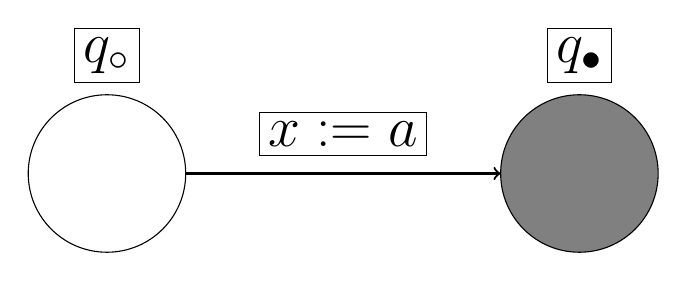
\begin{tikzpicture}
        \filldraw[fill=white, draw=black] (2,2) circle (1cm);
        \filldraw[fill=gray, draw=black] (8,2) circle (1cm);
        \node [draw] at (2,3.5) {\huge $q_{\circ}$};
        \node [draw] at (8,3.5) {\huge $q_{\bullet}$};
        \node [draw] at (5, 2.5) {\huge $x:=a$};
        \draw [thick, ->](3, 2) -- (7, 2);
    \end{tikzpicture}
    \caption{An example that shows a program graph of an assignment}
    \label{fig:tikz-program-graph-assignment}
\end{figure}
    \caption{An example that shows a program graph of an assignment}
    \label{fig:tikz-program-graph-assignment}
\end{figure}    
    \section{theory}\label{theory}

\subsection{Abstract Domains}\label{subsec:abstract_domains}

In the following sections we will describe the abstract domains of our value analysis.

\subsubsection{Abstract domain of strings as regular expressions}\label{subsubsec:abstract_domains_strings}

To represent the abstract domain of the family of SQL strings data types we have chosen regular expressions/languages.
Regular expressions/languages are chosen, as opposed to more powerful representations, for the decidable nature of inclusion and equality between them.

Let $REG$ denote the set of regular languages and
\begin{equation*}
    REG^{\leq n} = \{R \in REG \mid \forall w \in R : |w| \leq n\}.
\end{equation*}
In the following we do not distinguish between regular expressions and their languages.

In regards to abstract interpretation regulars expressions are not without their own quirks, as expressed in the following theorem.

The lattice of regular expressions $(REG, \subseteq, \cup, \cap)$ is not suited for abstract interpretation, as expressed by \autoref{thm:reg-lattice}.

\begin{restatable}{theorem}{reglattice}\label{thm:reg-lattice}
    $(REG, \subseteq, \cup, \cap)$ is a lattice, but not a complete one.
\end{restatable}

Thus we can not employ the Kleene fixed-point theorem to guarantee a fixed point and termination of our analysis.
We propose two solutions to overcome this limitation:
\begin{itemize}
    \item Limiting the size of the regulars expressions under consideration, this is sound in the case where the string data type which is abstracted over is fixed size;
    \item And to let the user define an abstract domain over the regular expressions that only contain finite elements.
\end{itemize}

To formalize the latter idea we introduce regular language partitions.

\begin{definition}
    Given a finite subset $REG^\subset \subset REG$ where $\bigcup REG^\subset = \Sigma^\star$.
    % todo Casper says: I am not sure if this restriction is useful.
    % and $\forall R_1, R_2 \in REG^\subset : R_1 \not\subset R_2 \land R_2 \not\subset R_1$.
    A regular language partition $p(REG^\subset)$ is a set where:
    \begin{itemize}
        % Casper says: I don't think the empty set in necessary.
        % \item $\emptyset \in p(REG^\subset)$,
        \item $\forall R \in REG^\subset : R \in p(REG^\subset)$,
        \item $\forall R_1, R_2 \in p(REG^\subset) : R_1 \cup R_2 \in p(REG^\subset)$,
        \item $\forall R_1, R_2 \in p(REG^\subset) : R_1 \cap R_2 \in p(REG^\subset)$.
    \end{itemize}
\end{definition}

% Tikzfigures
\begin{figure}
    \resizebox{7.5cm}{!}{
        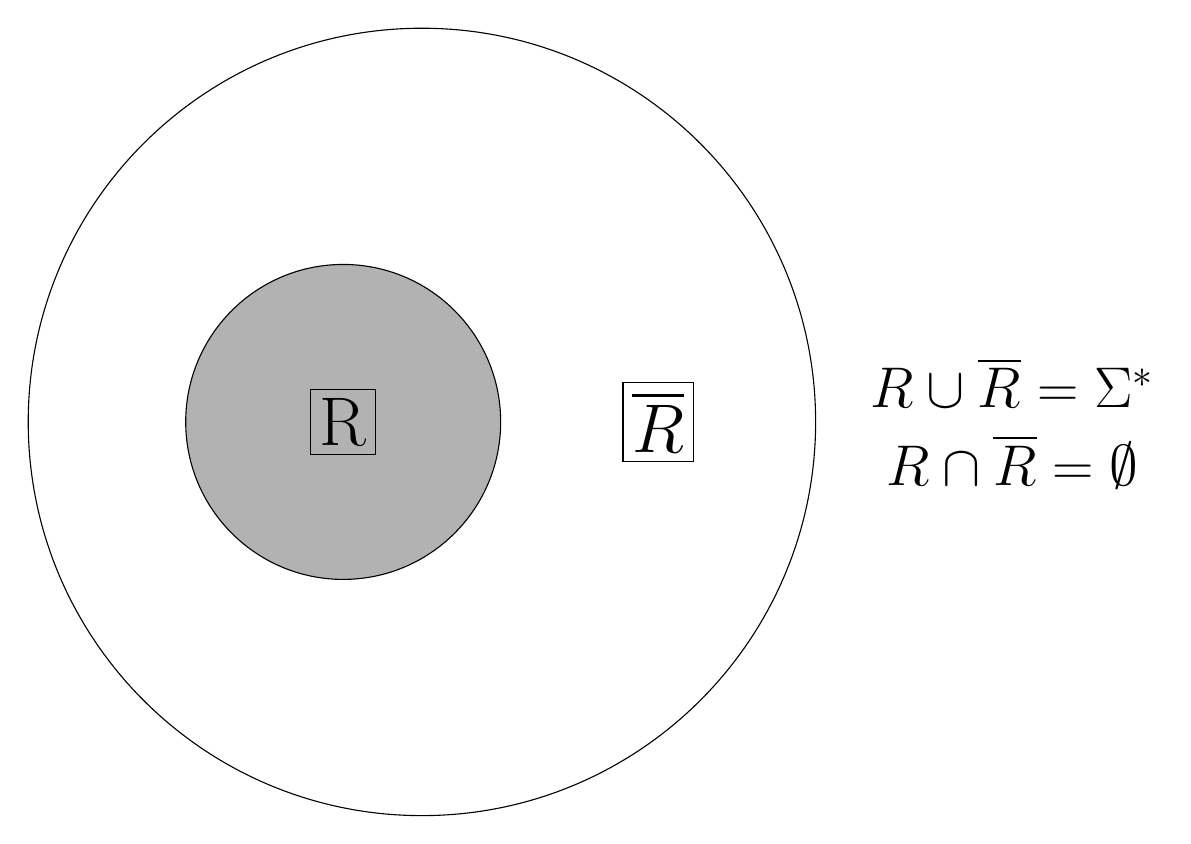
\begin{tikzpicture}
            \filldraw[fill=white, draw=black] (2,2) circle (5cm);
            \node [draw] at (5,2) {\Huge$\overline{R}$};
            \filldraw[fill=gray!60, draw=black] (1,2) circle (2cm);
            \node [draw] at (1,2) {\Huge R};
            \node at (9.5, 2.5) {\huge $R \cup \overline{R} = \Sigma^*$};
            \node at (9.5, 1.5) {\huge $R \cap \overline{R} = \emptyset$};
        \end{tikzpicture}
    }
    \caption{Regular language partition}
    \label{fig:tikz-reg-partition}
\end{figure}

\begin{figure}[!htb]
    \resizebox{6.5cm}{!}{
        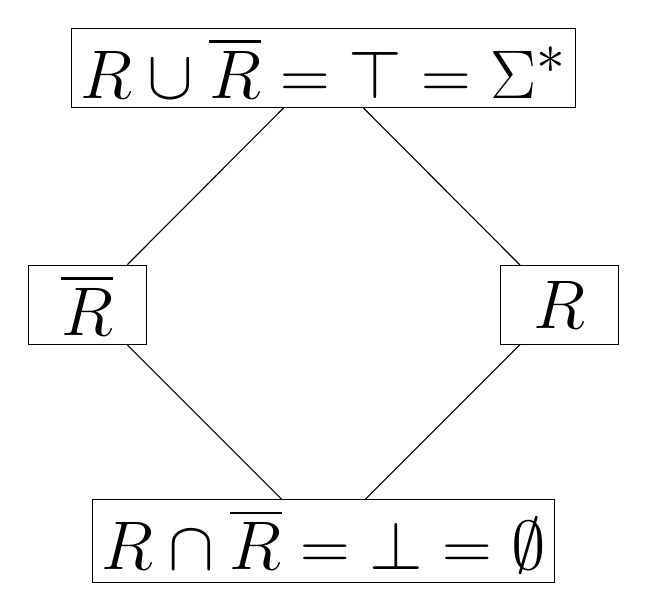
\begin{tikzpicture}[scale = 0.5]
            \usetikzlibrary{calc}
            \node (a) [state] {\Huge$R \cup \overline{R} = \top = \Sigma^*$};
            \node (b1) [state, shift={($(a.south)+(3cm, -2.5cm)$)}] {\Huge $R$};
            \node (b2) [state, shift={($(a.south)+(-3cm, -2.5cm)$)}]{\Huge $\overline{R}$};
            \node (c) [state, shift= {($(a.south) + (0cm, -5.5cm)$)}] {\Huge $R \cap \overline{R} = \bot = \emptyset$};
            \draw (a) to (b1);
            \draw (a) to (b2);
            \draw (b1) to (c);
            \draw (b2) to (c);
        \end{tikzpicture}
    }
    \caption{Regular language partition as a lattice}
    \label{fig:tikz-reg-partition-lattice}
\end{figure}

\begin{theorem}\label{thm:finite-reg-lattice}
    $(REG^{\leq n}, \subseteq, \cup, \cap)$ is a complete lattice.
\end{theorem}

\begin{theorem}\label{thm:reg-partition-lattice}
    $(p(REG^\subset), \subseteq, \cup, \cap)$ is a complete lattice.
\end{theorem}


\subsubsection{Abstract domain of numbers as linear inequalities}\label{subsubsec:abstract_domains_numbers}

To represent the abstract domain of the family of SQL number data types when have chosen compound linear inequalities, more specifically compound linear inequalities which are algorithmically solvable by \gls{lp}.
\gls{lp} solvable compound linear inequalities where chosen for the prevalence of \gls{lp} solvers.
%todo
\todo{
    Casper says: We probably need a better reasons.
    Maybe look into NLP, MINLP, CP, SDP and convex optimization.
}

Let $LP^n$ be the set of solutions to \gls{lp} solvable compound linear inequalities where $\mathbf{x} \in X \in LP \implies \mathbf{x} \in \mathbb{R}^n$.\todo{
    Casper says: I feel like the description is more awkward than it needs to be.
}
And Let $ILP^n$ be the set integer solutions with the same constraint as above.
\autoref{thm:lp-lattice} demonstrates a similar problem as the one we encounter with the lattice $(REG, \subseteq, \cup, \cap)$.

\begin{theorem}\label{thm:lp-lattice}
    For $\mathcal{LP}^n \in \{ILP^n, LP^n\}$ : $(\mathcal{LP}^n, \subseteq, \cup, \cap)$ is a lattice, but not a complete one.
\end{theorem}

Again we employ a similar solution:

\begin{definition}
    Given a finite subset $LP_\subset^n \subset LP^n$ where $\bigcup LP_\subset^n = \mathbb{R}^n$.
    A \gls{lp} partition $p(LP_\subset^n)$ is a set where:
    \begin{itemize}
        \item $\forall X \in LP_\subset^n : X \in p(LP_\subset^n)$,
        \item $\forall X, Y \in p(LP_\subset^n) : X \cup Y \in p(LP_\subset^n)$,
        \item $\forall X, Y \in p(LP_\subset^n) : X \cap Y \in p(LP_\subset^n)$,
    \end{itemize}
\end{definition}

\begin{definition}
    Given a finite subset $ILP_\subset^n \subset LP^n$ where $\bigcup LP_\subset^n = \mathbb{Z}^n$.
    A I\gls{lp} partition $p(ILP_\subset^n)$ is a set where:
    \begin{itemize}
        \item $\forall X \in ILP_\subset^n : X \in p(ILP_\subset^n)$,
        \item $\forall X, Y \in p(ILP_\subset^n) : X \cup Y \in p(ILP_\subset^n)$,
        \item $\forall X, Y \in p(ILP_\subset^n) : X \cap Y \in p(ILP_\subset^n)$,
    \end{itemize}
\end{definition}

\begin{theorem}\label{thm:lp-partition-lattice}
    For $\mathcal{LP} \in \{ILP, LP\}$ : $(p(\mathcal{LP}_\subset^n), \subseteq, \cup, \cap)$ is a complete lattice.
\end{theorem}

\todo[inline]{
    Casper says: At this point it seems that the concept of a partition can be generalized.
}

% Let $A$ denote $m \times n$ matrix, $\mathbf{x}$ a $n \times 1$ column vector of variable and $\mathbf{b}$ a $m \times 1$ column vector of constants, then the solutions to the linear inequality $A \mathbf{x} \leq \mathbf{b}$ can be described as:
% \begin{equation*}
%     \{\mathbf{x} \in \mathbb{R}^n \mid A \mathbf{x} \leq \mathbf{b} \}
% \end{equation*}
% For the set of solutions of linear inequalities $A \mathbf{x} \leq \mathbf{b}$ and $A' \mathbf{x}' \leq \mathbf{b}'$ where $\mathbf{x}$ and $\mathbf{x}'$ are of the same size, their union and intersection are given by:
% \begin{align*}
%     \{\mathbf{x} \in \mathbb{R}^n \mid A \mathbf{x} \leq \mathbf{b} \}
%     &\cup
%     \{\mathbf{x} \in \mathbb{R}^n \mid A' \mathbf{x} \leq \mathbf{b'} \} \\
%     &=
%     \{
%         \mathbf{x} \in \mathbb{R}^n \mid A \mathbf{x} \leq \mathbf{b}
%                                     \lor A' \mathbf{x} \leq \mathbf{b}'
%     \}
% \end{align*}
% and
% \begin{align*}
%     \{\mathbf{x} \in \mathbb{R}^n \mid A \mathbf{x} \leq \mathbf{b} \}
%     &\cap
%     \{\mathbf{x} \in \mathbb{R}^n \mid A' \mathbf{x} \leq \mathbf{b'} \} \\
%     &=
%     \{\mathbf{x} \in \mathbb{R}^n \mid \begin{bmatrix} A \\ A' \end{bmatrix}  \mathbf{x} \leq \begin{bmatrix} \mathbf{b} \\ \mathbf{b}' \end{bmatrix} \}
% \end{align*}














    \printglossary[type=\acronymtype]

    \printbibliography

    \appendices % You can use \appendix if you only have a single appendix
    %! Author = Runge
%! Date = 29-12-2023

\section{Proof of theorem \ref{thm:partition}}

\partition*

\begin{proof}
    \pf\
    \assume{
        $(S, \sqsubseteq, \sqcup, \sqcap)$ is a non-complete lattice and $X \subset S$ and $\bigsqcup X = \top$.
    }
    \prove{
        $(p(X), \sqsubseteq, \sqcup, \sqcap) \text{is a complete lattice}$.
    }
    \step{}{A nonempty finite lattice is a complete lattice.}
    \begin{proof}
        \pf\ Know property \cite{moller_statitc_nodate}.
    \end{proof}
    \step{}{$(p(X), \sqsubseteq, \sqcup, \sqcap)$ is a lattice.}
    \begin{proof}
        \step{poset}{$p(X)$ is a poset}
        \begin{proof}
            \step{poset-subset}{The subset of a poset is a poset under the same ordering relation.}
            \begin{proof}
                \pf\ Know property.\todo{source missing}
            \end{proof}
            \step{partition-subset}{$p(X) \subset S$}
            \begin{proof}
                \pf\ By the definition of a partition and lattices.
            \end{proof}
            \qedstep
            \begin{proof}
                \pf\ By \stepref{poset-subset} and \stepref{partition-subset}.
            \end{proof}
        \end{proof}
        \step{lattice}{$\forall x, y \in p(X) : x \sqcup y \in p(X) \land x \sqcap y \in p(X)$}
        \begin{proof}
            \pf\ By the definition of $p(X)$.
        \end{proof}
        \qedstep
        \begin{proof}
            % \pf\ By \stepref{poset} and \stepref{lattice}.
        \end{proof}
    \end{proof}
    \step{}{$p(X)$ is finite.}
    \begin{proof}
        \pf\ there is a finite number of ways to combine the elements of $X$ using $\sqcap$ and $\sqcup$ without repeating operations and repeated operations are idempotent, therefore $p(X)$ is finite.
    \end{proof}
    \qedstep
\end{proof}




\end{document}
